\section*{Введение}

% На данный момент в программных системах самым распространенным представлением информации, которая создается пользователем или демонстрируется ему, является текстовое представление. Оно удобно по многим причинам, но у него есть существенный недостаток - часто без дополнительного стилизирования текстовая информация слишком тяжело воспринимается. При отображении данных для пользователя необходимо явственным образом сохранять изначальную структуру информации. В большинстве случаев такое стилизирование сводится к форматированию текста, то есть добавлению или удалению не несущих информацxtbf{ию символов, другому преобразованию текста без изменения его семантики. Данное преобразование называется \textbf{pretty printing}.

С появлением первых языков программирования особую важность приобрели языковые процессоры. Языковой процессор (ЯП) -- это программное средство, принимающее на вход текст программы на некотором языке программирования и решающее определенную задачу над этим кодом. Языковые процессоры применяются для:
\begin{enumerate}
\item компиляции;
\item суперкомпиляции;
\item интерпретации;
\item статического анализа кода;
\item трансляции;
\item декомпиляции.
\end{enumerate}
Также используются в средствах интегрированной разработки программного обеспечения. Основные этапы работы языкового процессора представлены на рисунке~\ref{fig:languageProcessorFlow}.

\begin{wrapfigure}{r}{0.5\textwidth}
	\begin{center}
		\includegraphics[width=0.8\textwidth]{lanProcessorFlow}
	\end{center}
	\caption{Этапы работы ЯП}
	\label{fig:languageProcessorFlow}	
\end{wrapfigure}

Все задачи из приведенного списка, возможно, кроме компиляции и интерпретации, на промежуточном уровне обработки программного кода взаимодействуют с пользователем.

% Языковые процессоры являются большой и важной областью современной информатики. С появления первых языков программирования 
% Приведем лишь неполный перечень их видов:
% \begin{enumerate}
% \item компиляторы
% \item интерпретаторы
% \item средства статического анализа кода
% \item трансляторы
% \item декомпиляторы
% \item средства интегрированной разработки
% \end{enumerate}

В области языковых процессоров (ЯП) основной информацией, требующейся во взаимодействии с пользователем, являются программные коды. Внутри ЯП программы представляются древовидными структурами, а снаружи - с помощью текста. Поэтому практически каждый раз при создании нового ЯП, необходимо разработать и метод перевода синтаксического дерева в программный код на целевом языке.

% А эта необходимость поднимает вопрос использования соответствующей библиотеки. Такая библиотека должна предоставлять гибкие механизмы выбора раскладки текстовой информации по заданным параметрам, например, по указанию максимальной ширины текста. Выбор должен происходить среди вариантов, которые предоставлены библиотеке пользователем.

Рассмотрим небольшой пример. Пользователь задает условие вида: “последовательные операторы пишутся на одной строке, если помешаются в N символов. Иначе - на разных строках”.


\begin{figure}[h]
	\centering
	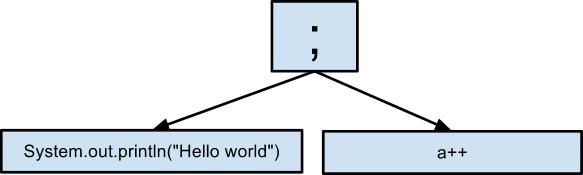
\includegraphics[width=0.8\textwidth]{seqTree}
	\caption{Последовательные операторы}
	\label{fig:seqImage}
\end{figure}

На рисунке~\ref{fig:seqImage} изображено синтаксическое дерево последовательности двух операторов. Такое дерево согласно заданному правилу может быть напечатано одним из двух вариантов (рисунки ~\ref{fig:seqCode1}, ~\ref{fig:seqCode2}).

\begin{figure}[h]
	\inputminted{c}{codes/seqCode1.java}
	\caption{Последовательные операторы. В строчку}
	\label{fig:seqCode1}
\end{figure}

\begin{figure}[h]
	\inputminted{c}{codes/seqCode2.java}
	\caption{Последовательные операторы. В несколько строк}
	\label{fig:seqCode2}
\end{figure}

Выбор происходит в зависимости от ширины вывода. Так при ширине равной 35 символов (длина строки “System.out.println(“Hello world”); ”), должен выбираться вариант, изображенный на рисунке~\ref{fig:seqCode2}, так как код на рисунке~\ref{fig:seqCode1} имеет ширину более 35 символов.
Могут быть заданы и более сложные условия. Рассмотрим другой пример. Пусть нам нужно текстовое представление синтаксического дерева конструкции If, и заданы нижеследующие шаблоны:

\begin{figure}[h]
	\inputminted{haskell}{codes/ifTemplate1.hs}
	\caption{Последовательные операторы. В строчку}
	\label{fig:ifTemplate1}
\end{figure}

\begin{figure}[h]
	\inputminted{haskell}{codes/ifTemplate2.hs}
	\caption{Последовательные операторы. В несколько строк}
	\label{fig:ifTemplate2}
\end{figure}

Причем вариант, изображенный на рисунке~\ref{fig:ifTemplate1} выбирается в случае, если условие и ветки могут быть напечатаны в одну строчку. Тогда для деревьев, представленных на рисунках \ref{fig:ifImage1} и \ref{fig:ifImage2}, будут напечатаны коды с рисунков \ref{fig:ifCode1} и \ref{fig:ifCode2} соответственно.

\begin{figure}[h!]
	\begin{minipage}[b]{0.65\linewidth}
		\centering
		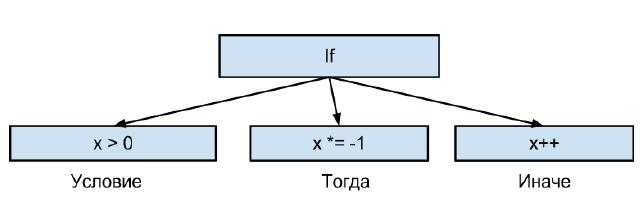
\includegraphics[width=\textwidth]{if1}
		\caption{}
		\label{fig:ifImage1}
	\end{minipage}
	\hspace{0.5cm}
	\begin{minipage}[b]{0.25\linewidth}
		\centering
		\inputminted{haskell}{codes/ifCode1.hs}
		\caption{asd}
		\label{fig:ifCode1}
	\end{minipage}
\end{figure}

\begin{figure}[h!]
	\begin{minipage}[b]{0.65\linewidth}
		\centering
		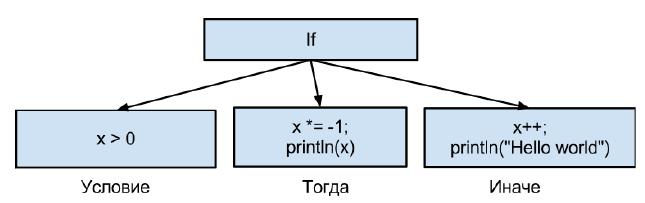
\includegraphics[width=\textwidth]{if2}
		\caption{asd}
		\label{fig:ifImage2}
	\end{minipage}
	\hspace{0.5cm}
	\begin{minipage}[b]{0.25\linewidth}
		\centering
		\inputminted{haskell}{codes/ifCode2.hs}
		\caption{asd}
		\label{fig:ifCode2}
	\end{minipage}
\end{figure}

%%bib testing
asadgdsgdsgsdagdsg asfadsfsdfsdfsdfs
sdfsadfsf
\cite{hughes}
\cite{swierstra}
\cite{olaf}
\cite{wadler}
\cite{peytonJones}
\cite{ocamlFormat}
sddfsdfasfasf